\subsection{Gyroskop}
Et gyroskop er et elektromekanisk apparat, som anvendes til at måle omdrejninger per sekund eller vinkelhastighed om en given akse, hvilket illustreres på \figref{fig:gyro}. Enhederne på data fra et gyroskop er henholdsvis revolutions per second (RPS) og $^\circ$/sekund. \newline
Et gyropskop kan give information om orienteringen eller navigationen af objektet, som sensoren optager data fra. Hvis et gyroskop eksempelvis drejes én omgang om egen akse i sekundet, vil den registrere en vinkelhastighed på 360 grader pr sekund. \citep{Sparkfun_gyro,Barbour2014}
\begin{figure}[H]
	\centering
	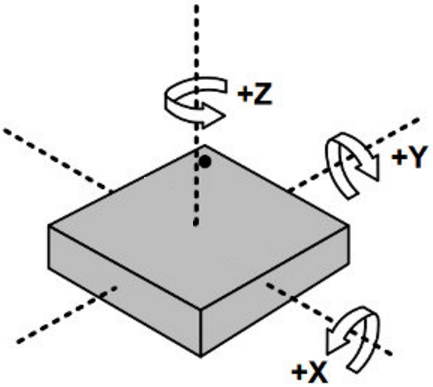
\includegraphics[scale=0.8]{figures/bProblemloesning/gyro.png}
	\caption{På figuren ses et gyroskops måling af rotation omkring x-, y- og z-aksen. \citep{Sparkfun_gyro} (Modificeret)}
	\label{fig:gyro}
\end{figure}

Alt afhængigt af formålet med at benyttes et gyroskop, findes der en række forskellige gyroskoper heriblandt vibrations-, elektrostatiske- og kernemagnetisk resonans gyroskoper. \citep{LuingeVeltink2005,TittertonWeston2004} Et gyroskop kan for eksempel registrere vinkelhastighed ved at anvende tyngdekræften og en lille indre masse \citep{Sparkfun_gyro,Barbour2014}. Hvis et gyroskop eksempelvis opsamler data ved cykling, mens det er placeret proximalt for den laterale malleolus, vil massen blive udsat for en roterende bevægelse omkring den horisontale akse. Massen vil blive henholdsvis tungere og lettere i processen på grund af ydre påvirkende kræfter, hvorfor outputtet vil komme til udtryk som en sinus-bølge. Outputtet er afhængig af tyngdekræftens påvirkning af massen, hvorfor et varierende output kræver en bevægelse.% Gyroskopet vil, uafhængigt af placering, have et fast output, som det vil vende tilbage til efter en bevægelse.
%Et gyroskop fungere ved at anvende inerti egenskaberne der opstår når et hjul spindes med en høj hastighed. Ved at hjulet fastholder den samme retning omkring aksen, kan impulsmomentmomentet, dets inertiprodukt samt hastighed være med til at definere en referenceretning. 
%De fundementale principper bag virkningen af et gyroskop er blandt andet det gyroskopiske inerti, som er når hjulet drejer om sin egen akse og står vinkelret på aksen. impulsmomentet som er fordelingen af en masse på et rotor, hvor vinkelhastigheden også har en betydning, og præcession som er rotationen omkring egen akse. 
%De signaler som opfanges af et accelerometrer, inkluderer ikke signaler fra den roterende akse og derfor kan en præcis orientering ikke opfanges. For at forbedre nøjagtigheden, kan man anvende gyroskoper som et supplement til accelerometre .
%Et gyroskop måler vinkelhastighed, hvor ændringen i orientering kan måles ved at integrere vinkelhastigheden på baggrund af en algoritme. \citep{LuingeVeltink2005}
%
\subsection{Sammenligning af accelerometer og gyroskop}
\textbf{Nyt forslag}
Acceleromteter er i stand til at måle accelerationen af et objekt, eksempelvis bevægelsen af et ben under gang, løb og cykling. Dette er er muligt idet denne sensor måler den kraft som eksempelvis et ben påvirkes med, ved en given bevægelse. Der vil derfor fremkomme karakteristika for en given bevægele for de respektive akser. Særligt gang og løb har en karakteristisk påvirkning af kroppen, hvilket yderligere fremgår af \secref{bevaegelse}. Accelerometeret vil derfor være fordelagtigt at benytte til en registrering af de pågælende bevægelser. \newline
Endvidere forefindes gyroskopet, som registrerer rotationen af et objekt om en given akse. Med antagelse om ideelle forhold vil det derfor være fordelagtigt at benytte et gyrooskop til registrering af cykling, idet denne bevægelse overordnet set er en cirkulær bevægelse om én akse. 

\textbf{Gammelt forslag} \newline
Den væsentligste forskel er, at et gyroskop kan måle rotation, hvilket et accelerometer ikke er i stand til. Accelerometret er fordelagtigt at bruge til at måle orientering af et stationært punkt i forhold til jordens overflade men under bevægelse bliver outputtet mere komplekst. For eksempel vil et accelerometer under frit fald vise 0. \citep{Goodrich2013,TittertonWeston2004,LuingeVeltink2005} \\
Et gyroskop reagerer ikke på vibration eller støj, hvilket et accelerometer kan opsamle som støj på signalet. Derudover reagerer et gyroskop hurtigt men dets output for hældningsvinkel vil blive mere ukorrekt over tid grundet usikkerhed i de enkelte målinger, hvorfor den akkumulerede vinkel ligeledes bliver mere ukorrekt. Et accelerometers respons er langsommere men mere præcis over tid. Igennem kalibrering, hvor hvert apparat assisterer til kalibreringen af den anden, vil de tilsammen kunne holdes korrekt på kort og lang sigt. \citep{Barbour2014,Brasca2011}